\documentclass[11pt,letterpaper]{article}

% =============================================================================
% PACKAGES
% =============================================================================
\usepackage[margin=1in]{geometry}
\usepackage{enumitem}
\usepackage{setspace}
\usepackage{graphicx}
\usepackage{xcolor}
\usepackage{tikz}
\usetikzlibrary{shapes.geometric, arrows.meta, positioning, fit, backgrounds, calc, decorations.pathreplacing, trees, matrix, shapes.multipart, shapes.symbols, shadows}
\usepackage{tcolorbox}
\usepackage{booktabs}
\usepackage{longtable}
\usepackage{array}
\usepackage{tabularx}
\usepackage{multirow}
\usepackage{fancyhdr}
\usepackage{titlesec}
\usepackage[colorlinks=true,linkcolor=blue!60!black,urlcolor=blue!60!black,citecolor=blue!60!black]{hyperref}
\usepackage{bookmark}
\usepackage{parskip}
\usepackage{float}
\usepackage{caption}
\usepackage{subcaption}
\usepackage{listings}
\usepackage{microtype}
\usepackage{textcomp}
\usepackage{amssymb}
\usepackage{amsmath}
\usepackage{pifont}

% =============================================================================
% CONFIGURATION
% =============================================================================
\setstretch{1.15}

% Define colors
\definecolor{primary}{RGB}{40, 80, 120}
\definecolor{secondary}{RGB}{70, 110, 150}
\definecolor{accent}{RGB}{180, 100, 50}
\definecolor{success}{RGB}{50, 130, 80}
\definecolor{warning}{RGB}{200, 150, 50}
\definecolor{critical}{RGB}{180, 60, 60}
\definecolor{lightgray}{RGB}{245, 245, 245}
\definecolor{darkgray}{RGB}{80, 80, 80}
\definecolor{systemcolor}{RGB}{200, 220, 255}
\definecolor{externalcolor}{RGB}{255, 235, 210}
\definecolor{usercolor}{RGB}{220, 255, 220}
\definecolor{datacolor}{RGB}{255, 230, 230}
\definecolor{servicecolor}{RGB}{240, 230, 255}
\definecolor{boundarycolor}{RGB}{180, 180, 180}
\definecolor{interfacecolor}{RGB}{255, 250, 200}

% Section formatting
\titleformat{\section}{\Large\bfseries\color{primary}}{\thesection}{1em}{}[\titlerule]
\titleformat{\subsection}{\large\bfseries\color{secondary}}{\thesubsection}{1em}{}
\titleformat{\subsubsection}{\normalsize\bfseries\color{darkgray}}{\thesubsubsection}{1em}{}

% Header/Footer
\pagestyle{fancy}
\fancyhf{}
\fancyhead[L]{\small\textcolor{darkgray}{Context Viewpoint Specification}}
\fancyhead[R]{\small\textcolor{darkgray}{Architecture Documentation}}
\fancyfoot[C]{\thepage}
\renewcommand{\headrulewidth}{0.4pt}

% Custom environments
\newtcolorbox{definitionbox}[1][]{
    colback=lightgray,
    colframe=primary,
    fonttitle=\bfseries,
    title=#1,
    boxrule=0.5pt,
    arc=2pt,
    left=8pt,
    right=8pt,
    top=6pt,
    bottom=6pt
}

\newtcolorbox{examplebox}[1][]{
    colback=white,
    colframe=secondary,
    fonttitle=\bfseries,
    title=#1,
    boxrule=0.5pt,
    arc=2pt,
    left=8pt,
    right=8pt,
    top=6pt,
    bottom=6pt
}

\newtcolorbox{warningbox}[1][]{
    colback=orange!5,
    colframe=accent,
    fonttitle=\bfseries,
    title=#1,
    boxrule=0.5pt,
    arc=2pt,
    left=8pt,
    right=8pt,
    top=6pt,
    bottom=6pt
}

\newtcolorbox{guidancebox}[1][]{
    colback=green!5,
    colframe=success,
    fonttitle=\bfseries,
    title=#1,
    boxrule=0.5pt,
    arc=2pt,
    left=8pt,
    right=8pt,
    top=6pt,
    bottom=6pt
}

\newtcolorbox{patternbox}[1][]{
    colback=blue!3,
    colframe=primary!70,
    fonttitle=\bfseries,
    title=#1,
    boxrule=0.5pt,
    arc=2pt,
    left=8pt,
    right=8pt,
    top=6pt,
    bottom=6pt
}

\newtcolorbox{contextbox}[1][]{
    colback=cyan!5,
    colframe=secondary,
    fonttitle=\bfseries,
    title=#1,
    boxrule=0.5pt,
    arc=2pt,
    left=8pt,
    right=8pt,
    top=6pt,
    bottom=6pt
}

\newtcolorbox{boundarybox}[1][]{
    colback=gray!5,
    colframe=boundarycolor,
    fonttitle=\bfseries,
    title=#1,
    boxrule=0.5pt,
    arc=2pt,
    left=8pt,
    right=8pt,
    top=6pt,
    bottom=6pt
}

% Listings configuration
\lstset{
    basicstyle=\ttfamily\small,
    backgroundcolor=\color{lightgray},
    frame=single,
    framerule=0.5pt,
    rulecolor=\color{darkgray},
    breaklines=true,
    captionpos=b,
    tabsize=2,
    showstringspaces=false,
    numbers=left,
    numberstyle=\tiny\color{darkgray},
    numbersep=5pt,
    xleftmargin=15pt,
    keywordstyle=\color{primary}\bfseries,
    commentstyle=\color{darkgray}\itshape,
    stringstyle=\color{success}
}

% Table column types
\newcolumntype{L}[1]{>{\raggedright\arraybackslash}p{#1}}
\newcolumntype{C}[1]{>{\centering\arraybackslash}p{#1}}
\newcolumntype{R}[1]{>{\raggedleft\arraybackslash}p{#1}}

% Custom commands
\newcommand{\cmark}{\ding{51}}
\newcommand{\xmark}{\ding{55}}

% =============================================================================
% DOCUMENT BEGIN
% =============================================================================
\begin{document}

% -----------------------------------------------------------------------------
% TITLE PAGE
% -----------------------------------------------------------------------------
% Avoid duplicate page anchors from titlepage/page counter resets
\hypersetup{pageanchor=false}

\begin{titlepage}
    \centering
    \vspace*{1.5cm}
    
    {\Huge\bfseries\color{primary} Context Viewpoint\par}
    \vspace{0.5cm}
    {\Large\color{secondary} Architecture Viewpoint Specification\par}
    \vspace{0.3cm}
    {\large\color{darkgray} System Environment, Boundaries \& External Interactions\par}
    
    \vspace{1.2cm}
    
    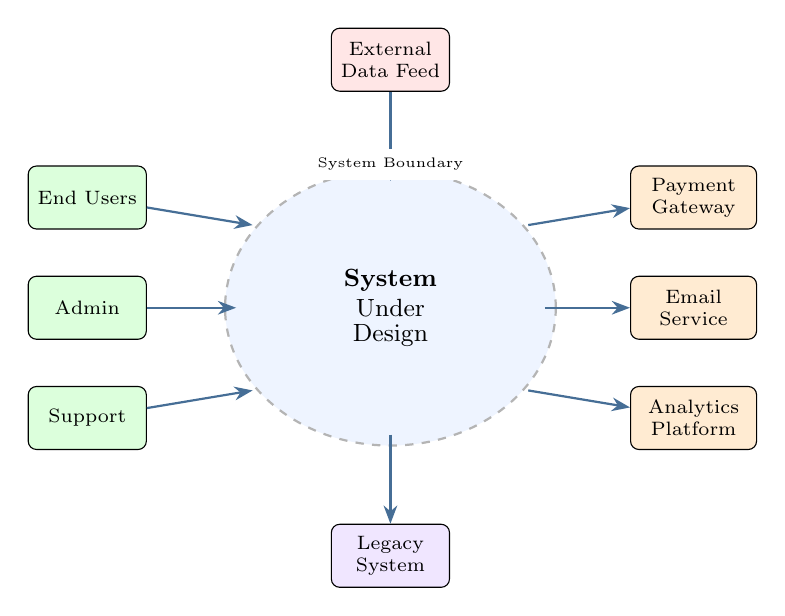
\begin{tikzpicture}[scale=0.7, every node/.style={align=center}]
        % System boundary
        \draw[thick, dashed, boundarycolor, fill=systemcolor!30] (0, 0) ellipse (3cm and 2.5cm);
        \node[font=\small\bfseries] at (0, 0.5) {System};
        \node[font=\small] at (0, 0) {Under};
        \node[font=\small] at (0, -0.5) {Design};
        
        % External users
        \node[draw, fill=usercolor, rounded corners=3pt, minimum width=1.5cm, minimum height=0.8cm, font=\scriptsize] (user1) at (-5.5, 2) {End Users};
        \node[draw, fill=usercolor, rounded corners=3pt, minimum width=1.5cm, minimum height=0.8cm, font=\scriptsize] (user2) at (-5.5, 0) {Admin};
        \node[draw, fill=usercolor, rounded corners=3pt, minimum width=1.5cm, minimum height=0.8cm, font=\scriptsize] (user3) at (-5.5, -2) {Support};
        
        % External systems
        \node[draw, fill=externalcolor, rounded corners=3pt, minimum width=1.6cm, minimum height=0.8cm, font=\scriptsize, align=center] (ext1) at (5.5, 2) {Payment\\Gateway};
        \node[draw, fill=externalcolor, rounded corners=3pt, minimum width=1.6cm, minimum height=0.8cm, font=\scriptsize, align=center] (ext2) at (5.5, 0) {Email\\Service};
        \node[draw, fill=externalcolor, rounded corners=3pt, minimum width=1.6cm, minimum height=0.8cm, font=\scriptsize, align=center] (ext3) at (5.5, -2) {Analytics\\Platform};
        
        % Data sources
        \node[draw, fill=datacolor, rounded corners=3pt, minimum width=1.5cm, minimum height=0.8cm, font=\scriptsize, align=center] (data1) at (0, 4.5) {External\\Data Feed};
        \node[draw, fill=servicecolor, rounded corners=3pt, minimum width=1.5cm, minimum height=0.8cm, font=\scriptsize, align=center] (data2) at (0, -4.5) {Legacy\\System};
        
        % Connections
        \draw[-{Stealth}, thick, secondary] (user1) -- (-2.5, 1.5);
        \draw[-{Stealth}, thick, secondary] (user2) -- (-2.8, 0);
        \draw[-{Stealth}, thick, secondary] (user3) -- (-2.5, -1.5);
        
        \draw[-{Stealth}, thick, secondary] (2.5, 1.5) -- (ext1);
        \draw[-{Stealth}, thick, secondary] (2.8, 0) -- (ext2);
        \draw[-{Stealth}, thick, secondary] (2.5, -1.5) -- (ext3);
        
        \draw[-{Stealth}, thick, secondary] (data1) -- (0, 2.3);
        \draw[-{Stealth}, thick, secondary] (0, -2.3) -- (data2);
        
        % Boundary label
        \node[font=\tiny, fill=white] at (0, 2.6) {System Boundary};
        
    \end{tikzpicture}
    
    \vspace{1.3cm}
    
    \begin{tabular}{ll}
        \textbf{Version:} & 2.0 \\
        \textbf{Status:} & Release \\
        \textbf{Classification:} & ISO/IEC/IEEE 42010 Compliant \\
        \textbf{Last Updated:} & \today \\
    \end{tabular}
    
    \vfill
    
    {\small Based on the Views and Beyond approach to software architecture documentation}
    
\end{titlepage}

\hypersetup{pageanchor=true}


% -----------------------------------------------------------------------------
% TABLE OF CONTENTS
% -----------------------------------------------------------------------------
\tableofcontents
\newpage

% =============================================================================
% SECTION: VIEWPOINT NAME
% =============================================================================
\section{Viewpoint Name}

\begin{definitionbox}[Viewpoint Identification]
\begin{tabular}{@{}L{3.5cm}L{10cm}@{}}
\textbf{Name:} & Context Viewpoint \\[0.5em]
\textbf{Synonyms:} & System Context View, Environmental View, External Interface View, Boundary View, Ecosystem View, Integration Context View \\[0.5em]
\textbf{Identifier:} & VP-CTX-001 \\[0.5em]
\textbf{Version:} & 2.0 \\
\end{tabular}
\end{definitionbox}

\subsection{Viewpoint Classification}

The Context Viewpoint defines the system's position within its broader environment, showing how the system interacts with external entities including users, systems, and services. While not explicitly defined as a style in the Views and Beyond approach, it represents essential architectural documentation that establishes scope and boundaries before detailed design. This viewpoint corresponds to the "context diagram" commonly used in system analysis and is foundational to IEEE 42010 architecture descriptions.

\begin{table}[H]
\centering
\caption{Viewpoint Classification Taxonomy}
\begin{tabular}{@{}L{4cm}L{10cm}@{}}
\toprule
\textbf{Attribute} & \textbf{Value} \\
\midrule
Style Family & Foundational / Cross-Cutting \\
Primary Focus & System Boundaries and External Relationships \\
Abstraction Level & High-Level / Strategic \\
Temporal Perspective & Static Environment Structure \\
Related Styles & Component-and-Connector (external), Use Case \\
IEEE 42010 Category & Context, Stakeholder Viewpoint \\
C4 Model Equivalent & System Context Diagram (Level 1) \\
\bottomrule
\end{tabular}
\end{table}

\subsection{Viewpoint Scope}

The Context Viewpoint encompasses the following aspects:

\begin{itemize}
    \item \textbf{System Boundary:} Clear definition of what is inside versus outside the system, establishing scope for architectural decisions.
    
    \item \textbf{External Actors:} Users, roles, and personas that interact with the system, including their goals and interaction patterns.
    
    \item \textbf{External Systems:} Other software systems, services, and platforms that the system integrates with or depends upon.
    
    \item \textbf{External Data Sources:} Data feeds, APIs, and information sources consumed by the system.
    
    \item \textbf{External Data Consumers:} Systems or entities that consume data or services provided by the system.
    
    \item \textbf{Environmental Constraints:} Technical, regulatory, organizational, and operational constraints from the environment.
    
    \item \textbf{Interface Contracts:} High-level specifications of how the system interacts with external entities.
    
    \item \textbf{Dependencies and Assumptions:} External dependencies and assumptions about the environment.
\end{itemize}

% =============================================================================
% SECTION: OVERVIEW
% =============================================================================
\section{Overview}

The Context Viewpoint provides a comprehensive picture of the system's operating environment and its position within a larger ecosystem. It is typically the first architectural view developed and serves as the foundation for more detailed architectural work.

\subsection{Purpose and Scope}

The primary purpose of this viewpoint is to establish clear boundaries around what the system is and what it is not, to identify all external entities the system must interact with, and to define the nature of those interactions. This shared understanding is essential for scope management, integration planning, and stakeholder alignment.

\begin{definitionbox}[Viewpoint Definition]
The Context Viewpoint defines the system's environment by identifying its boundaries, external actors, external systems, and the interactions between the system and its environment. It establishes what is in scope for the architecture, what external dependencies exist, and what interfaces the system must provide or consume. This viewpoint provides essential context for all other architectural views.
\end{definitionbox}

\subsection{Key Characteristics}

The Context Viewpoint exhibits several distinctive characteristics:

\textbf{Boundary Focus:} The primary concern is establishing clear boundaries between the system and its environment, defining what is "in" versus "out" of scope.

\textbf{High Abstraction:} The system is treated as a single entity (black box) with focus on external relationships rather than internal structure.

\textbf{Stakeholder Accessibility:} Designed to be understandable by all stakeholders including non-technical audiences, using simple notation and business terminology.

\textbf{Foundational Role:} Serves as the starting point for architecture work, establishing context before detailed design begins.

\textbf{Integration Emphasis:} Highlights all integration points and external dependencies that will require architectural attention.

\subsection{Relationship to Other Viewpoints}

The Context Viewpoint connects to other architectural viewpoints as a foundational reference:

\begin{table}[H]
\centering
\caption{Relationships to Other Viewpoints}
\begin{tabular}{@{}L{3.5cm}L{10.5cm}@{}}
\toprule
\textbf{Viewpoint} & \textbf{Relationship} \\
\midrule
Component-and-Connector & Context interfaces are realized by boundary components. External system connectors are detailed. \\
\addlinespace
Deployment & External systems inform deployment integration. Network boundaries align with context boundaries. \\
\addlinespace
Information/Data & External data sources feed data architecture. Data exchange formats are derived from context. \\
\addlinespace
Development & External APIs drive module interfaces. Integration code modules are identified. \\
\addlinespace
Security & Trust boundaries align with system boundaries. External actors drive access control design. \\
\addlinespace
Operational & External dependencies affect monitoring. SLAs with external systems are identified. \\
\bottomrule
\end{tabular}
\end{table}

\subsection{Context Architecture Overview}

\begin{figure}[H]
\centering
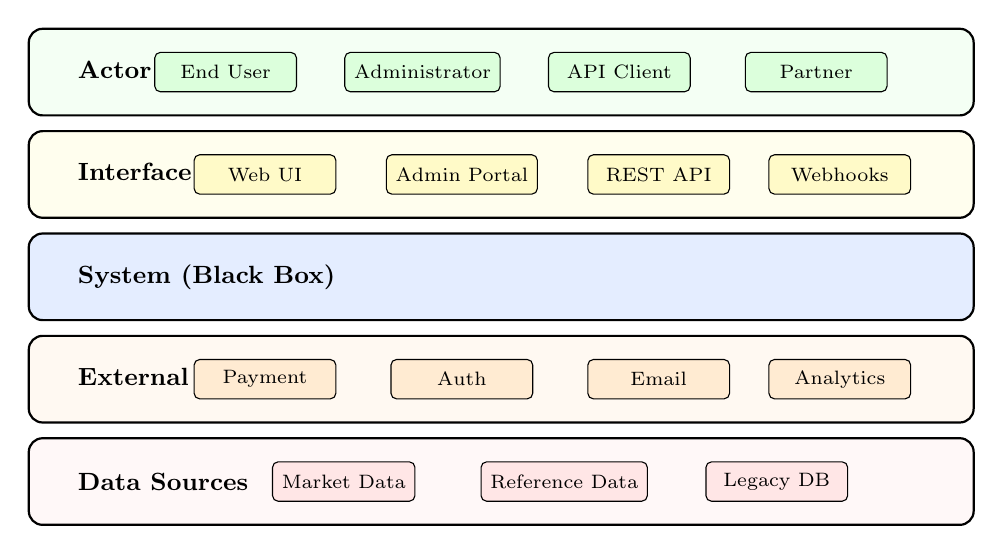
\begin{tikzpicture}[
    node distance=1cm and 1.5cm,
    layer/.style={draw, thick, rounded corners=5pt, minimum width=12cm, minimum height=1.1cm, font=\small},
    element/.style={draw, fill=systemcolor, rounded corners=2pt, minimum width=1.8cm, minimum height=0.5cm, font=\scriptsize},
]
    % Layers
    \node[layer, fill=usercolor!30] (actors) at (0, 3.5) {};
    \node[font=\small\bfseries, anchor=west] at (-5.5, 3.5) {Actor Layer};
    
    \node[layer, fill=interfacecolor!30] (interfaces) at (0, 2.2) {};
    \node[font=\small\bfseries, anchor=west] at (-5.5, 2.2) {Interface Layer};
    
    \node[layer, fill=systemcolor!50] (system) at (0, 0.9) {};
    \node[font=\small\bfseries, anchor=west] at (-5.5, 0.9) {System (Black Box)};
    
    \node[layer, fill=externalcolor!30] (external) at (0, -0.4) {};
    \node[font=\small\bfseries, anchor=west] at (-5.5, -0.4) {External Systems};
    
    \node[layer, fill=datacolor!30] (data) at (0, -1.7) {};
    \node[font=\small\bfseries, anchor=west] at (-5.5, -1.7) {Data Sources};
    
    % Actor elements
    \node[element, fill=usercolor] at (-3.5, 3.5) {End User};
    \node[element, fill=usercolor] at (-1, 3.5) {Administrator};
    \node[element, fill=usercolor] at (1.5, 3.5) {API Client};
    \node[element, fill=usercolor] at (4, 3.5) {Partner};
    
    % Interface elements
    \node[element, fill=interfacecolor] at (-3, 2.2) {Web UI};
    \node[element, fill=interfacecolor] at (-0.5, 2.2) {Admin Portal};
    \node[element, fill=interfacecolor] at (2, 2.2) {REST API};
    \node[element, fill=interfacecolor] at (4.3, 2.2) {Webhooks};
    
    % External elements
    \node[element, fill=externalcolor] at (-3, -0.4) {Payment};
    \node[element, fill=externalcolor] at (-0.5, -0.4) {Auth};
    \node[element, fill=externalcolor] at (2, -0.4) {Email};
    \node[element, fill=externalcolor] at (4.3, -0.4) {Analytics};
    
    % Data elements
    \node[element, fill=datacolor] at (-2, -1.7) {Market Data};
    \node[element, fill=datacolor] at (0.8, -1.7) {Reference Data};
    \node[element, fill=datacolor] at (3.5, -1.7) {Legacy DB};
    
\end{tikzpicture}
\caption{Context Architecture Layers}
\end{figure}

% =============================================================================
% SECTION: CONCERNS
% =============================================================================
\section{Concerns}

This section enumerates the architectural concerns that the Context Viewpoint is designed to address.

\subsection{Primary Concerns}

\begin{enumerate}[label=\textbf{C\arabic*:}, leftmargin=2.5em]
    \item \textbf{System Scope and Boundaries}
    \begin{itemize}[nosep]
        \item What functionality is included in the system?
        \item What is explicitly out of scope?
        \item Where are the system boundaries?
        \item What are the boundary interfaces?
        \item How are scope decisions documented and communicated?
    \end{itemize}
    
    \item \textbf{External Actors and Users}
    \begin{itemize}[nosep]
        \item Who are the human users of the system?
        \item What roles and personas exist?
        \item What are their goals and needs?
        \item How do they interact with the system?
        \item What are their technical capabilities?
    \end{itemize}
    
    \item \textbf{External System Dependencies}
    \begin{itemize}[nosep]
        \item What external systems does the system depend on?
        \item What services do they provide?
        \item What are the availability and reliability characteristics?
        \item What happens when dependencies are unavailable?
        \item What are the contractual relationships?
    \end{itemize}
    
    \item \textbf{Integration Points}
    \begin{itemize}[nosep]
        \item What integration interfaces exist?
        \item What protocols and formats are used?
        \item What are synchronous vs asynchronous integrations?
        \item What data is exchanged?
        \item What transformation or mapping is required?
    \end{itemize}
    
    \item \textbf{Data Exchange}
    \begin{itemize}[nosep]
        \item What data flows into the system?
        \item What data flows out of the system?
        \item What are the data volumes and frequencies?
        \item What data quality expectations exist?
        \item How is data ownership managed?
    \end{itemize}
    
    \item \textbf{Environmental Constraints}
    \begin{itemize}[nosep]
        \item What technical constraints exist (platforms, protocols)?
        \item What regulatory constraints apply?
        \item What organizational policies affect the system?
        \item What geographical or jurisdictional constraints exist?
        \item What time-based constraints apply?
    \end{itemize}
    
    \item \textbf{Security Boundaries}
    \begin{itemize}[nosep]
        \item What are the trust boundaries?
        \item What authentication/authorization exists at boundaries?
        \item What data protection applies at interfaces?
        \item What compliance requirements affect external interfaces?
        \item How are security incidents with external parties handled?
    \end{itemize}
    
    \item \textbf{Service Level Expectations}
    \begin{itemize}[nosep]
        \item What availability expectations exist for external interfaces?
        \item What performance expectations exist?
        \item What SLAs govern external dependencies?
        \item How are service levels monitored?
        \item What happens when SLAs are breached?
    \end{itemize}
    
    \item \textbf{Evolution and Change}
    \begin{itemize}[nosep]
        \item How stable are external interfaces?
        \item What versioning strategies are used?
        \item How are breaking changes communicated?
        \item What backward compatibility is required?
        \item How are new integrations added?
    \end{itemize}
    
    \item \textbf{Assumptions and Risks}
    \begin{itemize}[nosep]
        \item What assumptions are made about the environment?
        \item What risks arise from external dependencies?
        \item What contingency plans exist?
        \item How are assumptions validated?
        \item What external factors could disrupt the system?
    \end{itemize}
\end{enumerate}

\subsection{Concern-Quality Attribute Mapping}

\begin{table}[H]
\centering
\caption{Concern to Quality Attribute Mapping}
\small
\begin{tabular}{@{}L{3cm}C{1cm}C{1cm}C{1cm}C{1cm}C{1cm}C{1cm}C{1cm}C{1cm}@{}}
\toprule
\textbf{Concern} & \rotatebox{60}{\textbf{Interop.}} & \rotatebox{60}{\textbf{Security}} & \rotatebox{60}{\textbf{Availability}} & \rotatebox{60}{\textbf{Modtic.}} & \rotatebox{60}{\textbf{Perform.}} & \rotatebox{60}{\textbf{Scalability}} & \rotatebox{60}{\textbf{Usability}} & \rotatebox{60}{\textbf{Compliance}} \\
\midrule
Scope/Boundaries & $\circ$ & $\bullet$ & $\circ$ & $\bullet$ & -- & -- & $\circ$ & $\circ$ \\
External Actors & $\circ$ & $\bullet$ & $\circ$ & $\circ$ & $\circ$ & $\circ$ & $\bullet$ & $\circ$ \\
Dependencies & $\bullet$ & $\circ$ & $\bullet$ & $\circ$ & $\bullet$ & $\circ$ & -- & $\circ$ \\
Integration & $\bullet$ & $\circ$ & $\circ$ & $\bullet$ & $\bullet$ & $\bullet$ & -- & $\circ$ \\
Data Exchange & $\bullet$ & $\bullet$ & $\circ$ & $\circ$ & $\bullet$ & $\bullet$ & -- & $\bullet$ \\
Constraints & $\circ$ & $\circ$ & $\circ$ & $\circ$ & $\circ$ & $\circ$ & $\circ$ & $\bullet$ \\
Security Bounds & $\circ$ & $\bullet$ & $\circ$ & $\circ$ & $\circ$ & -- & -- & $\bullet$ \\
Service Levels & $\circ$ & -- & $\bullet$ & -- & $\bullet$ & $\bullet$ & $\circ$ & $\circ$ \\
Evolution & $\bullet$ & $\circ$ & $\circ$ & $\bullet$ & -- & $\circ$ & -- & -- \\
Assumptions & $\circ$ & $\circ$ & $\bullet$ & $\circ$ & $\circ$ & $\circ$ & -- & $\circ$ \\
\bottomrule
\multicolumn{9}{l}{\footnotesize $\bullet$ = Primary impact, $\circ$ = Secondary impact, -- = Minimal impact}
\end{tabular}
\end{table}

% =============================================================================
% SECTION: ANTI-CONCERNS
% =============================================================================
\section{Anti-Concerns}

Understanding what the Context Viewpoint is \emph{not} appropriate for helps stakeholders avoid misapplying this viewpoint.

\subsection{Out of Scope Topics}

\begin{enumerate}[label=\textbf{AC\arabic*:}, leftmargin=2.5em]
    \item \textbf{Internal System Structure}
    \begin{itemize}[nosep]
        \item Component decomposition within the system
        \item Internal module dependencies
        \item Internal data flows
        \item Implementation technologies
        \item Internal algorithms and logic
    \end{itemize}
    
    \item \textbf{Detailed Interface Specifications}
    \begin{itemize}[nosep]
        \item API endpoint definitions
        \item Message schema details
        \item Protocol specifications
        \item Error handling details
        \item Rate limiting configurations
    \end{itemize}
    
    \item \textbf{Deployment Architecture}
    \begin{itemize}[nosep]
        \item Server and infrastructure topology
        \item Container orchestration
        \item Network configuration
        \item Cloud resource allocation
        \item Environment configurations
    \end{itemize}
    
    \item \textbf{Process and Thread Design}
    \begin{itemize}[nosep]
        \item Concurrency architecture
        \item Thread pool configurations
        \item Process communication
        \item Synchronization mechanisms
        \item Runtime behavior
    \end{itemize}
    
    \item \textbf{Operational Procedures}
    \begin{itemize}[nosep]
        \item Monitoring configurations
        \item Alerting rules
        \item Incident response procedures
        \item Deployment pipelines
        \item Runbook details
    \end{itemize}
\end{enumerate}

\begin{warningbox}[Common Misapplications]
Avoid using the Context Viewpoint for:

\begin{itemize}[nosep]
    \item Documenting internal component structure (use C\&C Viewpoint)
    \item Specifying API contracts in detail (use Interface Specifications)
    \item Defining deployment topology (use Deployment Viewpoint)
    \item Detailing data models (use Information Viewpoint)
    \item Specifying process architecture (use Process Viewpoint)
\end{itemize}
\end{warningbox}

% =============================================================================
% SECTION: TYPICAL STAKEHOLDERS
% =============================================================================
\section{Typical Stakeholders}

The Context Viewpoint serves a broad audience as it establishes foundational understanding of the system.

\subsection{Primary Stakeholders}

\begin{table}[H]
\centering
\caption{Primary Stakeholder Analysis}
\small
\begin{tabular}{@{}L{2.6cm}L{3.6cm}L{7cm}@{}}
\toprule
\textbf{Stakeholder} & \textbf{Role Description} & \textbf{Primary Interests} \\
\midrule
Project Sponsors & Fund and authorize project & Scope clarity, business alignment, risk understanding \\
\addlinespace
Product Managers & Define product direction & Feature scope, user identification, market positioning \\
\addlinespace
Software Architects & Design system structure & Integration requirements, constraints, dependencies \\
\addlinespace
Business Analysts & Define requirements & User roles, business processes, external touchpoints \\
\addlinespace
System Integrators & Connect systems together & Integration points, protocols, data formats \\
\addlinespace
Enterprise Architects & Manage system portfolio & Ecosystem fit, standards compliance, redundancy \\
\bottomrule
\end{tabular}
\end{table}

\subsection{Secondary Stakeholders}

\begin{table}[H]
\centering
\caption{Secondary Stakeholder Analysis}
\small
\begin{tabular}{@{}L{2.6cm}L{3.6cm}L{7cm}@{}}
\toprule
\textbf{Stakeholder} & \textbf{Role Description} & \textbf{Primary Interests} \\
\midrule
Development Teams & Build the system & External API understanding, integration work scope \\
\addlinespace
Security Teams & Protect system assets & Trust boundaries, external attack surface, compliance \\
\addlinespace
Operations Teams & Run production systems & External dependencies, monitoring boundaries, SLAs \\
\addlinespace
Legal/Compliance & Ensure regulatory compliance & Data flows, jurisdictions, regulatory boundaries \\
\addlinespace
Partner Organizations & External system owners & Integration requirements, responsibilities, timelines \\
\addlinespace
End Users & Use the system & Understanding system capabilities and limitations \\
\bottomrule
\end{tabular}
\end{table}

\subsection{Stakeholder Concern Matrix}

\begin{table}[H]
\centering
\caption{Stakeholder-Concern Responsibility Matrix}
\footnotesize
\begin{tabular}{@{}L{2cm}C{0.8cm}C{0.8cm}C{0.8cm}C{0.8cm}C{0.8cm}C{0.8cm}C{0.8cm}C{0.8cm}C{0.8cm}C{0.8cm}@{}}
\toprule
& \rotatebox{60}{\textbf{Scope}} & \rotatebox{60}{\textbf{Actors}} & \rotatebox{60}{\textbf{Depend.}} & \rotatebox{60}{\textbf{Integr.}} & \rotatebox{60}{\textbf{Data}} & \rotatebox{60}{\textbf{Constr.}} & \rotatebox{60}{\textbf{Security}} & \rotatebox{60}{\textbf{SLAs}} & \rotatebox{60}{\textbf{Evolut.}} & \rotatebox{60}{\textbf{Risk}} \\
\midrule
Sponsor & A & I & I & I & I & A & I & A & I & A \\
Product Mgr & R & R & C & C & C & C & I & C & R & C \\
Architect & R & C & R & R & R & R & R & R & R & R \\
Bus. Analyst & C & R & C & C & R & C & I & C & C & C \\
Integrator & C & I & A & A & A & C & C & C & A & C \\
Security & C & C & C & C & C & C & A & C & C & C \\
\bottomrule
\multicolumn{11}{l}{\footnotesize R = Responsible, A = Accountable, C = Consulted, I = Informed}
\end{tabular}
\end{table}

% =============================================================================
% SECTION: MODEL TYPES
% =============================================================================
\section{Model Types}

The Context Viewpoint employs several complementary model types to capture different aspects of the system's environment.

\subsection{Model Type Catalog}

\begin{enumerate}[label=\textbf{MT\arabic*:}, leftmargin=2.5em]
    \item \textbf{System Context Diagram}
    \begin{itemize}[nosep]
        \item \textit{Purpose:} Show system as black box with all external entities
        \item \textit{Primary Elements:} System, actors, external systems, data flows
        \item \textit{Key Relationships:} Interacts-with, sends-to, receives-from
        \item \textit{Typical Notation:} C4 Context, custom diagrams, DFD Level 0
    \end{itemize}
    
    \item \textbf{Actor Catalog}
    \begin{itemize}[nosep]
        \item \textit{Purpose:} Document all users and their characteristics
        \item \textit{Primary Elements:} Actors, roles, goals, capabilities
        \item \textit{Key Relationships:} Plays-role, has-goal, interacts-via
        \item \textit{Typical Notation:} Tables, personas, user profiles
    \end{itemize}
    
    \item \textbf{External System Inventory}
    \begin{itemize}[nosep]
        \item \textit{Purpose:} Catalog all external system dependencies
        \item \textit{Primary Elements:} Systems, owners, interfaces, SLAs
        \item \textit{Key Relationships:} Depends-on, provides, consumes
        \item \textit{Typical Notation:} Tables, dependency matrices
    \end{itemize}
    
    \item \textbf{Interface Summary}
    \begin{itemize}[nosep]
        \item \textit{Purpose:} Overview of all external interfaces
        \item \textit{Primary Elements:} Interfaces, protocols, data types
        \item \textit{Key Relationships:} Exposes, consumes, exchanges
        \item \textit{Typical Notation:} Interface tables, API summaries
    \end{itemize}
    
    \item \textbf{Data Flow Overview}
    \begin{itemize}[nosep]
        \item \textit{Purpose:} Show high-level data movement across boundaries
        \item \textit{Primary Elements:} Data sources, sinks, flow directions
        \item \textit{Key Relationships:} Flows-from, flows-to, transforms
        \item \textit{Typical Notation:} DFD Level 0, data flow diagrams
    \end{itemize}
    
    \item \textbf{Trust Boundary Diagram}
    \begin{itemize}[nosep]
        \item \textit{Purpose:} Show security boundaries and trust zones
        \item \textit{Primary Elements:} Trust zones, boundaries, crossing points
        \item \textit{Key Relationships:} Contains, crosses, authenticates
        \item \textit{Typical Notation:} Security zone diagrams, threat models
    \end{itemize}
    
    \item \textbf{Constraint Catalog}
    \begin{itemize}[nosep]
        \item \textit{Purpose:} Document environmental constraints
        \item \textit{Primary Elements:} Constraints, sources, impacts
        \item \textit{Key Relationships:} Constrains, derives-from, affects
        \item \textit{Typical Notation:} Tables, constraint matrices
    \end{itemize}
    
    \item \textbf{Dependency Map}
    \begin{itemize}[nosep]
        \item \textit{Purpose:} Visualize critical dependencies and risks
        \item \textit{Primary Elements:} Dependencies, criticality, fallback
        \item \textit{Key Relationships:} Depends-on, falls-back-to, critical-for
        \item \textit{Typical Notation:} Dependency graphs, risk matrices
    \end{itemize}
    
    \item \textbf{Ecosystem Map}
    \begin{itemize}[nosep]
        \item \textit{Purpose:} Show system within broader organizational ecosystem
        \item \textit{Primary Elements:} Systems, domains, relationships
        \item \textit{Key Relationships:} Part-of, integrates-with, replaces
        \item \textit{Typical Notation:} Enterprise architecture diagrams
    \end{itemize}
\end{enumerate}

\subsection{Model Type Relationships}

\begin{figure}[H]
\centering
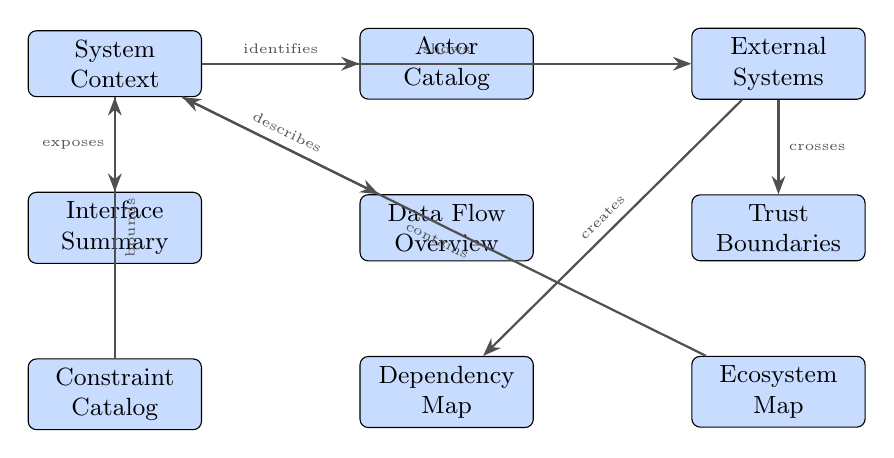
\begin{tikzpicture}[
    node distance=1.2cm and 2cm,
    model/.style={draw, fill=systemcolor, rounded corners=3pt, minimum width=2.2cm, minimum height=0.7cm, font=\small, align=center},
    arrow/.style={-{Stealth}, thick, darkgray}
]
    % Nodes - top row
    \node[model, align=center] (context) {System\\Context};
    \node[model, right=2cm of context, align=center] (actors) {Actor\\Catalog};
    \node[model, right=2cm of actors, align=center] (systems) {External\\Systems};
    
    % Nodes - middle row
    \node[model, below=1.2cm of context, align=center] (interface) {Interface\\Summary};
    \node[model, below=1.2cm of actors, align=center] (dataflow) {Data Flow\\Overview};
    \node[model, below=1.2cm of systems, align=center] (trust) {Trust\\Boundaries};
    
    % Nodes - bottom row
    \node[model, below=1.2cm of interface, align=center] (constraint) {Constraint\\Catalog};
    \node[model, below=1.2cm of dataflow, align=center] (dependency) {Dependency\\Map};
    \node[model, below=1.2cm of trust, align=center] (ecosystem) {Ecosystem\\Map};
    
    % Arrows
    \draw[arrow] (context) -- (actors) node[midway, above, font=\tiny] {identifies};
    \draw[arrow] (context) -- (systems) node[midway, above, font=\tiny] {shows};
    \draw[arrow] (context) -- (interface) node[midway, left, font=\tiny] {exposes};
    \draw[arrow] (context) -- (dataflow) node[midway, above, sloped, font=\tiny] {describes};
    \draw[arrow] (systems) -- (trust) node[midway, right, font=\tiny] {crosses};
    \draw[arrow] (systems) -- (dependency) node[midway, above, sloped, font=\tiny] {creates};
    \draw[arrow] (constraint) -- (context) node[midway, below, sloped, font=\tiny] {bounds};
    \draw[arrow] (ecosystem) -- (context) node[midway, below, sloped, font=\tiny] {contains};
\end{tikzpicture}
\caption{Model Type Dependency Relationships}
\end{figure}

% =============================================================================
% SECTION: MODEL LANGUAGES
% =============================================================================
\section{Model Languages}

For each model type, specific languages, notations, and techniques are prescribed.

\subsection{Context Diagram Notation}

\begin{figure}[H]
\centering
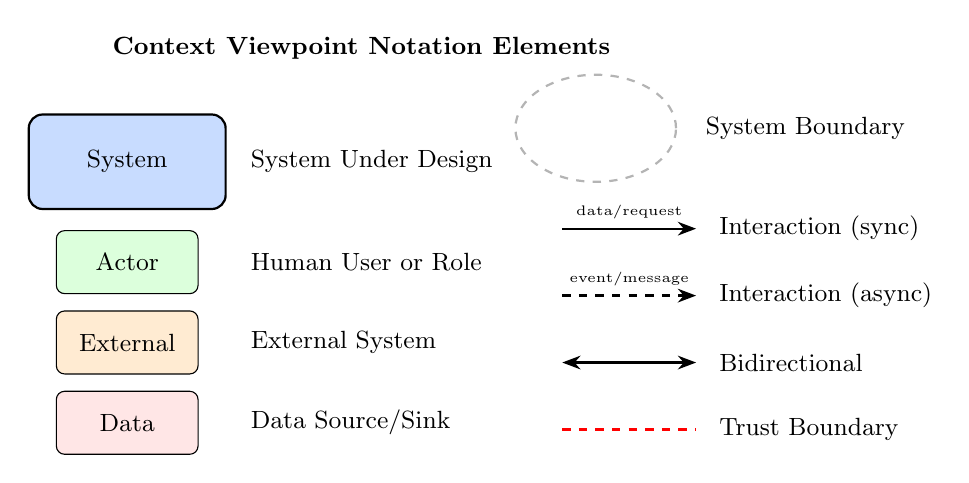
\begin{tikzpicture}[scale=0.85]
    % Legend title
    \node[font=\small\bfseries] at (0, 5) {Context Viewpoint Notation Elements};
    
    % System
    \node[draw, thick, fill=systemcolor, rounded corners=5pt, minimum width=2.5cm, minimum height=1.2cm] at (-3.5, 3.3) {};
    \node[font=\small] at (-3.5, 3.3) {System};
    \node[right, font=\small] at (-1.8, 3.3) {System Under Design};
    
    % Actor
    \node[draw, fill=usercolor, rounded corners=3pt, minimum width=1.8cm, minimum height=0.8cm] at (-3.5, 1.8) {};
    \node[font=\small] at (-3.5, 1.8) {Actor};
    \node[right, font=\small] at (-1.8, 1.8) {Human User or Role};
    
    % External System
    \node[draw, fill=externalcolor, rounded corners=3pt, minimum width=1.8cm, minimum height=0.8cm] at (-3.5, 0.6) {};
    \node[font=\small] at (-3.5, 0.6) {External};
    \node[right, font=\small] at (-1.8, 0.6) {External System};
    
    % Data Source
    \node[draw, fill=datacolor, rounded corners=3pt, minimum width=1.8cm, minimum height=0.8cm] at (-3.5, -0.6) {};
    \node[font=\small] at (-3.5, -0.6) {Data};
    \node[right, font=\small] at (-1.8, -0.6) {Data Source/Sink};
    
    % Boundary
    \draw[thick, dashed, boundarycolor] (3.5, 3.8) ellipse (1.2cm and 0.8cm);
    \node[right, font=\small] at (5, 3.8) {System Boundary};
    
    % Sync interaction
    \draw[-{Stealth}, thick] (3, 2.3) -- (5, 2.3);
    \node[above, font=\tiny] at (4, 2.3) {data/request};
    \node[right, font=\small] at (5.2, 2.3) {Interaction (sync)};
    
    % Async interaction
    \draw[-{Stealth}, thick, dashed] (3, 1.3) -- (5, 1.3);
    \node[above, font=\tiny] at (4, 1.3) {event/message};
    \node[right, font=\small] at (5.2, 1.3) {Interaction (async)};
    
    % Bidirectional
    \draw[{Stealth}-{Stealth}, thick] (3, 0.3) -- (5, 0.3);
    \node[right, font=\small] at (5.2, 0.3) {Bidirectional};
    
    % Trust boundary
    \draw[thick, red, dashed] (3, -0.7) -- (5, -0.7);
    \node[right, font=\small] at (5.2, -0.7) {Trust Boundary};
    
\end{tikzpicture}
\caption{Context Viewpoint Notation Legend}
\end{figure}

\subsection{Actor Classification}

\begin{table}[H]
\centering
\caption{Actor Type Classification}
\small
\begin{tabular}{@{}L{2.5cm}L{4cm}L{6.5cm}@{}}
\toprule
\textbf{Actor Type} & \textbf{Description} & \textbf{Examples} \\
\midrule
End User & Direct users of system functionality & Customers, members, subscribers \\
\addlinespace
Administrator & Users managing system configuration & System admins, tenant admins \\
\addlinespace
Operator & Users monitoring and operating system & DevOps, support staff \\
\addlinespace
API Consumer & Automated clients using APIs & Partner systems, mobile apps \\
\addlinespace
Data Provider & Sources that feed data to system & Market data feeds, IoT devices \\
\addlinespace
Auditor & Users reviewing system activity & Compliance officers, auditors \\
\bottomrule
\end{tabular}
\end{table}

\subsection{External System Classification}

\begin{table}[H]
\centering
\caption{External System Type Classification}
\small
\begin{tabular}{@{}L{2.5cm}L{4cm}L{6.5cm}@{}}
\toprule
\textbf{System Type} & \textbf{Description} & \textbf{Examples} \\
\midrule
SaaS Service & Third-party cloud services & Stripe, SendGrid, Auth0 \\
\addlinespace
Enterprise System & Internal organizational systems & ERP, CRM, HR systems \\
\addlinespace
Legacy System & Older systems being integrated & Mainframe, older databases \\
\addlinespace
Partner System & External partner integrations & Supplier APIs, partner portals \\
\addlinespace
Data Provider & External data sources & Bloomberg, weather services \\
\addlinespace
Infrastructure & Platform infrastructure services & AWS, Azure, DNS, CDN \\
\bottomrule
\end{tabular}
\end{table}

\subsection{Interface Classification}

\begin{table}[H]
\centering
\caption{Interface Type Classification}
\small
\begin{tabular}{@{}L{2.5cm}L{2cm}L{2.5cm}L{5.5cm}@{}}
\toprule
\textbf{Interface Type} & \textbf{Direction} & \textbf{Style} & \textbf{Use Cases} \\
\midrule
REST API & Bidirectional & Sync & CRUD operations, resource access \\
\addlinespace
GraphQL & Bidirectional & Sync & Flexible queries, mobile apps \\
\addlinespace
gRPC & Bidirectional & Sync & Service-to-service, high performance \\
\addlinespace
Webhook & Outbound & Async & Event notifications, callbacks \\
\addlinespace
Message Queue & Both & Async & Event streaming, decoupling \\
\addlinespace
File Transfer & Both & Batch & Bulk data exchange, reports \\
\addlinespace
Web UI & Inbound & Sync & Human user interaction \\
\addlinespace
Database Link & Both & Sync & Legacy integration, replication \\
\bottomrule
\end{tabular}
\end{table}

\subsection{Tabular Specifications}

\subsubsection{Actor Specification Table}

\begin{table}[H]
\centering
\caption{Example Actor Specification Format}
\small
\begin{tabular}{@{}L{2cm}L{2.2cm}L{3cm}L{2.5cm}L{2.5cm}@{}}
\toprule
\textbf{Actor} & \textbf{Type} & \textbf{Goals} & \textbf{Interface} & \textbf{Volume} \\
\midrule
Customer & End User & Browse, purchase, track orders & Web UI, Mobile & 100K DAU \\
Store Admin & Administrator & Manage inventory, pricing & Admin Portal & 500 users \\
Partner API & API Consumer & Sync inventory, orders & REST API & 1M req/day \\
Warehouse & Operator & Fulfill orders, manage stock & Internal App & 50 users \\
\bottomrule
\end{tabular}
\end{table}

\subsubsection{External System Specification Table}

\begin{table}[H]
\centering
\caption{Example External System Specification Format}
\small
\begin{tabular}{@{}L{2cm}L{2cm}L{2.5cm}L{2cm}L{2cm}L{2cm}@{}}
\toprule
\textbf{System} & \textbf{Type} & \textbf{Purpose} & \textbf{Protocol} & \textbf{SLA} & \textbf{Owner} \\
\midrule
Stripe & SaaS & Payment processing & REST & 99.99\% & Stripe Inc \\
Auth0 & SaaS & Authentication & OIDC & 99.99\% & Okta \\
SAP ERP & Enterprise & Order sync & RFC & 99.5\% & Finance IT \\
Kafka & Internal & Event streaming & Kafka & 99.9\% & Platform \\
\bottomrule
\end{tabular}
\end{table}

\subsubsection{Constraint Specification Table}

\begin{table}[H]
\centering
\caption{Example Constraint Specification Format}
\small
\begin{tabular}{@{}L{2.5cm}L{2cm}L{4cm}L{4cm}@{}}
\toprule
\textbf{Constraint} & \textbf{Type} & \textbf{Description} & \textbf{Impact} \\
\midrule
GDPR & Regulatory & EU data protection rules & Data handling, consent, deletion \\
PCI-DSS & Regulatory & Payment card security & Payment interface isolation \\
Corporate SSO & Technical & Must use corporate identity & Auth0 integration required \\
AWS Only & Organizational & Cloud provider restriction & Limits service choices \\
\bottomrule
\end{tabular}
\end{table}

% =============================================================================
% SECTION: VIEWPOINT METAMODELS
% =============================================================================
\section{Viewpoint Metamodels}

This section defines the conceptual metamodel underlying the Context Viewpoint.

\subsection{Core Metamodel}

\begin{figure}[H]
\centering
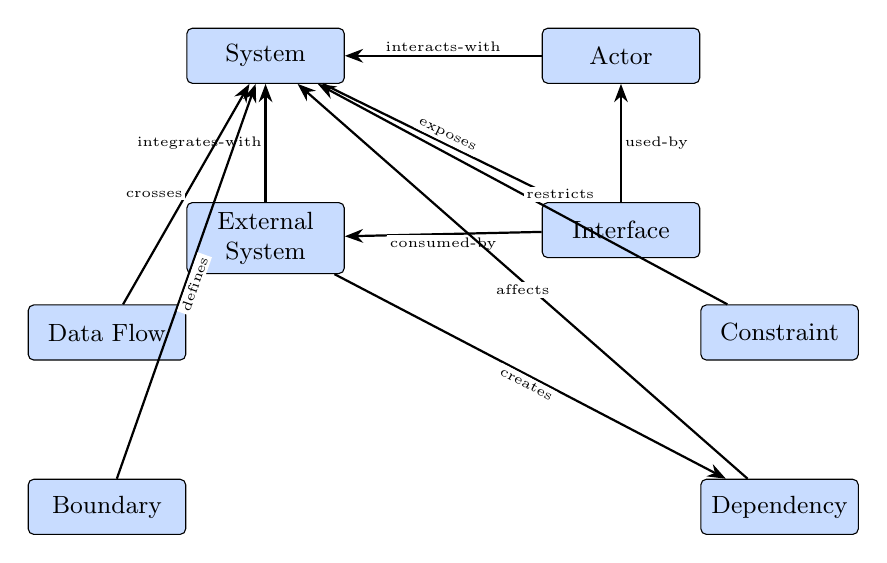
\begin{tikzpicture}[
    node distance=1.3cm and 2cm,
    entity/.style={draw, fill=systemcolor, rounded corners=2pt, minimum width=2cm, minimum height=0.7cm, font=\small, align=center},
    arrow/.style={-{Stealth}, thick},
    label/.style={font=\tiny, fill=white, inner sep=1pt}
]
    % Main entities
    \node[entity] (system) {System};
    \node[entity, right=2.5cm of system] (actor) {Actor};
    \node[entity, below=1.5cm of system, align=center] (external) {External\\System};
    \node[entity, below=1.5cm of actor] (interface) {Interface};
    \node[entity, below left=2.8cm and 0cm of system] (dataflow) {Data Flow};
    \node[entity, below right=2.8cm and 0cm of actor] (constraint) {Constraint};
    \node[entity, below=1.5cm of dataflow] (boundary) {Boundary};
    \node[entity, below=1.5cm of constraint] (dependency) {Dependency};
    
    % Relationships
    \draw[arrow] (actor) -- (system) node[label, midway, above] {interacts-with};
    \draw[arrow] (external) -- (system) node[label, midway, left] {integrates-with};
    \draw[arrow] (system) -- (interface) node[label, midway, above, sloped] {exposes};
    \draw[arrow] (interface) -- (actor) node[label, midway, right] {used-by};
    \draw[arrow] (interface) -- (external) node[label, midway, below] {consumed-by};
    \draw[arrow] (dataflow) -- (system) node[label, midway, left] {crosses};
    \draw[arrow] (constraint) -- (system) node[label, midway, right] {restricts};
    \draw[arrow] (boundary) -- (system) node[label, midway, below, sloped] {defines};
    \draw[arrow] (external) -- (dependency) node[label, midway, below, sloped] {creates};
    \draw[arrow] (dependency) -- (system) node[label, midway, below] {affects};
    
\end{tikzpicture}
\caption{Context Viewpoint Core Metamodel}
\end{figure}

\subsection{Entity Definitions}

\begin{definitionbox}[Entity: System]
\textbf{Definition:} The system under design, treated as a black box in the context view, representing the scope of the architectural effort.

\textbf{Attributes:}
\begin{itemize}[nosep]
    \item \texttt{systemId}: Unique identifier
    \item \texttt{name}: System name
    \item \texttt{description}: System purpose and scope
    \item \texttt{version}: Current version
    \item \texttt{status}: Development status (planned, in-development, production)
    \item \texttt{owner}: Owning organization or team
    \item \texttt{domain}: Business domain
    \item \texttt{criticality}: Business criticality level
    \item \texttt{scopeStatement}: What is in/out of scope
\end{itemize}

\textbf{Constraints:}
\begin{itemize}[nosep]
    \item System scope must be clearly defined
    \item System must have identified owner
    \item System must have at least one external interaction
\end{itemize}
\end{definitionbox}

\begin{definitionbox}[Entity: Actor]
\textbf{Definition:} A human user, role, or persona that interacts with the system to achieve goals.

\textbf{Attributes:}
\begin{itemize}[nosep]
    \item \texttt{actorId}: Unique identifier
    \item \texttt{name}: Actor name or role title
    \item \texttt{type}: Actor type (end-user, admin, operator, auditor)
    \item \texttt{description}: Actor characteristics and responsibilities
    \item \texttt{goals}: What the actor wants to achieve
    \item \texttt{frequency}: How often they interact
    \item \texttt{volume}: Expected number of this actor type
    \item \texttt{technicalLevel}: Technical sophistication
    \item \texttt{accessLevel}: Authorization level
    \item \texttt{interfaces}: How they access the system
\end{itemize}

\textbf{Constraints:}
\begin{itemize}[nosep]
    \item Each actor must have defined goals
    \item Actor must have at least one interface for interaction
    \item Access levels must be defined for authorization
\end{itemize}
\end{definitionbox}

\begin{definitionbox}[Entity: External System]
\textbf{Definition:} A software system, service, or platform outside the system boundary that the system interacts with.

\textbf{Attributes:}
\begin{itemize}[nosep]
    \item \texttt{systemId}: Unique identifier
    \item \texttt{name}: System name
    \item \texttt{type}: System type (SaaS, enterprise, legacy, partner)
    \item \texttt{description}: System purpose and capabilities
    \item \texttt{owner}: Organization or vendor that owns it
    \item \texttt{contact}: Technical contact information
    \item \texttt{protocol}: Communication protocol(s)
    \item \texttt{dataExchanged}: Data types exchanged
    \item \texttt{direction}: Inbound, outbound, or bidirectional
    \item \texttt{sla}: Service level agreement
    \item \texttt{availability}: Expected availability
    \item \texttt{documentation}: Link to API/integration docs
\end{itemize}

\textbf{Constraints:}
\begin{itemize}[nosep]
    \item External system must have identified owner
    \item Integration protocol must be specified
    \item Critical dependencies must have SLAs
    \item Fallback behavior must be defined for critical dependencies
\end{itemize}
\end{definitionbox}

\begin{definitionbox}[Entity: Interface]
\textbf{Definition:} A point of interaction between the system and external entities, defining how communication occurs.

\textbf{Attributes:}
\begin{itemize}[nosep]
    \item \texttt{interfaceId}: Unique identifier
    \item \texttt{name}: Interface name
    \item \texttt{type}: Interface type (REST API, Web UI, Message Queue, etc.)
    \item \texttt{description}: Interface purpose
    \item \texttt{direction}: Provided or consumed
    \item \texttt{protocol}: Communication protocol
    \item \texttt{dataFormat}: Data format (JSON, XML, Protobuf)
    \item \texttt{authentication}: Authentication mechanism
    \item \texttt{authorization}: Authorization model
    \item \texttt{versioning}: Versioning strategy
    \item \texttt{documentation}: Link to detailed specification
\end{itemize}

\textbf{Constraints:}
\begin{itemize}[nosep]
    \item All external interfaces must have authentication
    \item Interfaces must have versioning strategy
    \item Public interfaces must have documentation
\end{itemize}
\end{definitionbox}

\begin{definitionbox}[Entity: Data Flow]
\textbf{Definition:} A movement of data across the system boundary, characterizing what data is exchanged with external entities.

\textbf{Attributes:}
\begin{itemize}[nosep]
    \item \texttt{flowId}: Unique identifier
    \item \texttt{name}: Flow name
    \item \texttt{description}: Flow purpose
    \item \texttt{source}: Origin of data
    \item \texttt{destination}: Destination of data
    \item \texttt{dataType}: Type of data being transferred
    \item \texttt{volume}: Expected data volume
    \item \texttt{frequency}: How often data flows
    \item \texttt{sensitivity}: Data sensitivity classification
    \item \texttt{transformation}: Any transformation required
    \item \texttt{latencyRequirement}: Maximum acceptable delay
\end{itemize}

\textbf{Constraints:}
\begin{itemize}[nosep]
    \item Sensitive data flows must be encrypted
    \item Data flows must have defined owners
    \item Cross-boundary flows must be documented
\end{itemize}
\end{definitionbox}

\begin{definitionbox}[Entity: Constraint]
\textbf{Definition:} A limitation or requirement imposed on the system by its environment that must be accommodated.

\textbf{Attributes:}
\begin{itemize}[nosep]
    \item \texttt{constraintId}: Unique identifier
    \item \texttt{name}: Constraint name
    \item \texttt{type}: Constraint type (regulatory, technical, organizational, business)
    \item \texttt{description}: Detailed description
    \item \texttt{source}: Where the constraint comes from
    \item \texttt{rationale}: Why this constraint exists
    \item \texttt{impact}: How it affects the system
    \item \texttt{compliance}: How compliance is verified
    \item \texttt{exceptions}: Any approved exceptions
    \item \texttt{reviewDate}: When constraint should be reviewed
\end{itemize}

\textbf{Constraints:}
\begin{itemize}[nosep]
    \item Regulatory constraints must have compliance verification
    \item Constraints must have documented rationale
    \item Exceptions must be formally approved
\end{itemize}
\end{definitionbox}

\begin{definitionbox}[Entity: Boundary]
\textbf{Definition:} A demarcation that separates the system from its environment, defining scope and responsibility limits.

\textbf{Attributes:}
\begin{itemize}[nosep]
    \item \texttt{boundaryId}: Unique identifier
    \item \texttt{name}: Boundary name
    \item \texttt{type}: Boundary type (system, trust, organizational, network)
    \item \texttt{description}: What the boundary separates
    \item \texttt{inside}: What is inside the boundary
    \item \texttt{outside}: What is outside the boundary
    \item \texttt{crossingPoints}: Interfaces that cross the boundary
    \item \texttt{controls}: Security or governance controls at boundary
\end{itemize}

\textbf{Constraints:}
\begin{itemize}[nosep]
    \item Trust boundaries must have security controls
    \item All boundary crossings must be through defined interfaces
    \item Boundary scope must be unambiguous
\end{itemize}
\end{definitionbox}

\begin{definitionbox}[Entity: Dependency]
\textbf{Definition:} A reliance on an external system or service that creates risk if the dependency is unavailable or changes.

\textbf{Attributes:}
\begin{itemize}[nosep]
    \item \texttt{dependencyId}: Unique identifier
    \item \texttt{name}: Dependency name
    \item \texttt{target}: External system depended upon
    \item \texttt{type}: Dependency type (runtime, build-time, data)
    \item \texttt{criticality}: How critical (critical, important, convenience)
    \item \texttt{impact}: Impact if dependency unavailable
    \item \texttt{fallback}: Fallback behavior or alternative
    \item \texttt{monitoring}: How dependency health is monitored
    \item \texttt{sla}: Required service level
    \item \texttt{riskMitigation}: Risk mitigation strategies
\end{itemize}

\textbf{Constraints:}
\begin{itemize}[nosep]
    \item Critical dependencies must have fallback strategies
    \item Dependencies must have monitoring
    \item High-risk dependencies must have mitigation plans
\end{itemize}
\end{definitionbox}

\subsection{Relationship Definitions}

\begin{table}[H]
\centering
\caption{Metamodel Relationship Definitions}
\small
\begin{tabular}{@{}L{2.3cm}L{1.8cm}L{1.8cm}L{7.5cm}@{}}
\toprule
\textbf{Relationship} & \textbf{Source} & \textbf{Target} & \textbf{Description} \\
\midrule
interacts-with & Actor & System & Actor uses the system \\
\addlinespace
integrates-with & External & System & External system connects to system \\
\addlinespace
exposes & System & Interface & System provides this interface \\
\addlinespace
consumes & System & Interface & System uses external interface \\
\addlinespace
used-by & Interface & Actor & Interface is accessed by actor \\
\addlinespace
consumed-by & Interface & External & Interface is used by external system \\
\addlinespace
crosses & Data Flow & Boundary & Data moves across boundary \\
\addlinespace
restricts & Constraint & System & Constraint limits system \\
\addlinespace
defines & Boundary & System & Boundary establishes system scope \\
\addlinespace
creates & External & Dependency & External system creates dependency \\
\bottomrule
\end{tabular}
\end{table}

% =============================================================================
% SECTION: CONFORMING NOTATIONS
% =============================================================================
\section{Conforming Notations}

Several existing notations and modeling approaches align with the Context Viewpoint.

\subsection{C4 Model - Context Diagram}

The C4 Model's System Context diagram is a primary conforming notation for this viewpoint.

\textbf{Elements:} Person (user), Software System (external), System Boundary.

\textbf{Conformance Level:} Full conformance for context modeling.

\textbf{Tool Support:} Structurizr, PlantUML-C4, draw.io C4 shapes.

\subsection{UML Use Case Diagrams}

UML Use Case diagrams show actors and their interactions with system use cases.

\textbf{Elements:} Actors, Use Cases, System Boundary, Associations.

\textbf{Conformance Level:} Partial - focuses on functionality rather than systems.

\textbf{Tool Support:} Enterprise Architect, Visual Paradigm, StarUML.

\subsection{Data Flow Diagrams (Level 0)}

Context-level DFDs show the system with external entities and data flows.

\textbf{Elements:} Process (system), External Entity, Data Flow.

\textbf{Conformance Level:} Good for data-centric systems.

\textbf{Tool Support:} Lucidchart, Visio, draw.io.

\subsection{ArchiMate}

ArchiMate provides comprehensive enterprise architecture notation including context elements.

\textbf{Elements:} Business Actors, Application Components, Relationships.

\textbf{Conformance Level:} Full - designed for enterprise context.

\textbf{Tool Support:} Archi, Sparx EA, BiZZdesign.

\subsection{Notation Comparison}

\begin{table}[H]
\centering
\caption{Context Notation Comparison}
\small
\begin{tabular}{@{}L{2.5cm}C{1.2cm}C{1.2cm}C{1.2cm}C{1.2cm}C{1.2cm}C{1.2cm}@{}}
\toprule
\textbf{Feature} & \rotatebox{60}{\textbf{C4}} & \rotatebox{60}{\textbf{UML UC}} & \rotatebox{60}{\textbf{DFD}} & \rotatebox{60}{\textbf{ArchiMate}} & \rotatebox{60}{\textbf{BPMN}} & \rotatebox{60}{\textbf{Custom}} \\
\midrule
System boundary & $\bullet$ & $\bullet$ & $\bullet$ & $\bullet$ & $\circ$ & $\bullet$ \\
Human actors & $\bullet$ & $\bullet$ & $\circ$ & $\bullet$ & $\bullet$ & $\bullet$ \\
External systems & $\bullet$ & $\circ$ & $\bullet$ & $\bullet$ & $\circ$ & $\bullet$ \\
Data flows & $\circ$ & -- & $\bullet$ & $\bullet$ & $\bullet$ & $\bullet$ \\
Trust boundaries & $\circ$ & -- & -- & $\bullet$ & -- & $\bullet$ \\
Constraints & -- & -- & -- & $\bullet$ & -- & $\bullet$ \\
Simplicity & $\bullet$ & $\bullet$ & $\bullet$ & $\circ$ & $\circ$ & $\bullet$ \\
Standardized & $\circ$ & $\bullet$ & $\circ$ & $\bullet$ & $\bullet$ & -- \\
\bottomrule
\multicolumn{7}{l}{\footnotesize $\bullet$ = Strong support, $\circ$ = Limited support, -- = Not applicable}
\end{tabular}
\end{table}

% =============================================================================
% SECTION: MODEL CORRESPONDENCE RULES
% =============================================================================
\section{Model Correspondence Rules}

Model correspondence rules define how elements in context models relate to elements in other architectural views.

\subsection{Component-and-Connector View Correspondence}

\begin{definitionbox}[Correspondence Rule CR-01: Interface to Component Mapping]
\textbf{Rule:} Every external interface in the context view must be realized by a boundary component in the C\&C view.

\textbf{Formal Expression:}
\begin{center}
$\forall i \in Interfaces_{Context} : \exists c \in Components_{C\&C} : realizes(c, i)$
\end{center}

\textbf{Rationale:} Ensures context interfaces are architecturally implemented.

\textbf{Verification:} Interface-to-component traceability matrix.
\end{definitionbox}

\begin{definitionbox}[Correspondence Rule CR-02: External System to Connector Mapping]
\textbf{Rule:} Every external system integration must have a corresponding connector in the C\&C view.

\textbf{Formal Expression:}
\begin{center}
$\forall ext \in ExternalSystems : \exists conn \in Connectors : connects(conn, ext)$
\end{center}

\textbf{Rationale:} Ensures integrations are architecturally visible.

\textbf{Verification:} Integration architecture review.
\end{definitionbox}

\subsection{Deployment View Correspondence}

\begin{definitionbox}[Correspondence Rule CR-03: Boundary to Network Mapping]
\textbf{Rule:} System boundaries should align with network security boundaries in deployment.

\textbf{Formal Expression:}
\begin{center}
$\forall b \in TrustBoundaries_{Context} : \exists n \in NetworkZones_{Deploy} : aligns(b, n)$
\end{center}

\textbf{Rationale:} Ensures logical boundaries are physically enforced.

\textbf{Verification:} Network architecture review.
\end{definitionbox}

\subsection{Security View Correspondence}

\begin{definitionbox}[Correspondence Rule CR-04: Actor to Access Control Mapping]
\textbf{Rule:} Every actor type must have corresponding roles and permissions in security design.

\textbf{Formal Expression:}
\begin{center}
$\forall a \in Actors : \exists R \subseteq Roles : authorizes(R, a)$
\end{center}

\textbf{Rationale:} Ensures actors have defined access controls.

\textbf{Verification:} Role mapping review.
\end{definitionbox}

% =============================================================================
% SECTION: OPERATIONS ON VIEWS
% =============================================================================
\section{Operations on Views}

This section defines methods for creating, interpreting, analyzing, and maintaining context views.

\subsection{Creation Methods}

\subsubsection{View Development Process}

\begin{guidancebox}[Step 1: Define System Scope]
\begin{enumerate}[nosep]
    \item Review project charter and business case
    \item Identify system purpose and objectives
    \item Document what is explicitly in scope
    \item Document what is explicitly out of scope
    \item Get stakeholder agreement on scope boundaries
\end{enumerate}
\end{guidancebox}

\begin{guidancebox}[Step 2: Identify External Actors]
\begin{enumerate}[nosep]
    \item List all human user types
    \item Define roles and personas
    \item Document actor goals and needs
    \item Estimate actor volumes
    \item Identify actor technical capabilities
\end{enumerate}
\end{guidancebox}

\begin{guidancebox}[Step 3: Identify External Systems]
\begin{enumerate}[nosep]
    \item List all systems the system must integrate with
    \item Categorize by type (SaaS, enterprise, legacy, partner)
    \item Identify system owners and contacts
    \item Document integration purposes
    \item Assess availability and reliability
\end{enumerate}
\end{guidancebox}

\begin{guidancebox}[Step 4: Define Interfaces]
\begin{enumerate}[nosep]
    \item List all interfaces the system will expose
    \item List all external interfaces the system will consume
    \item Document protocols and data formats
    \item Define authentication/authorization requirements
    \item Plan versioning strategies
\end{enumerate}
\end{guidancebox}

\begin{guidancebox}[Step 5: Map Data Flows]
\begin{enumerate}[nosep]
    \item Identify all data entering the system
    \item Identify all data leaving the system
    \item Document data types and volumes
    \item Classify data sensitivity
    \item Identify transformation requirements
\end{enumerate}
\end{guidancebox}

\begin{guidancebox}[Step 6: Document Constraints]
\begin{enumerate}[nosep]
    \item Identify regulatory constraints
    \item Document technical constraints
    \item List organizational constraints
    \item Assess business constraints
    \item Document constraint impacts
\end{enumerate}
\end{guidancebox}

\begin{guidancebox}[Step 7: Analyze Dependencies and Risks]
\begin{enumerate}[nosep]
    \item Assess dependency criticality
    \item Identify single points of failure
    \item Document fallback strategies
    \item Plan dependency monitoring
    \item Create risk mitigation plans
\end{enumerate}
\end{guidancebox}

\subsubsection{Integration Patterns}

\begin{patternbox}[Pattern: API Gateway]
\textbf{Context:} Multiple external consumers need to access system capabilities.

\textbf{Solution:} Single entry point that routes, authenticates, and rate-limits external requests.

\textbf{Benefits:}
\begin{itemize}[nosep]
    \item Centralized authentication and authorization
    \item Rate limiting and throttling
    \item Request/response transformation
    \item API versioning support
    \item Monitoring and analytics
\end{itemize}

\textbf{Use When:} Multiple external API consumers, need for centralized control.
\end{patternbox}

\begin{patternbox}[Pattern: Anti-Corruption Layer]
\textbf{Context:} Integrating with legacy or external system with incompatible model.

\textbf{Solution:} Translation layer that converts between system's domain model and external model.

\textbf{Benefits:}
\begin{itemize}[nosep]
    \item Protects domain model integrity
    \item Isolates external model changes
    \item Enables gradual migration
    \item Simplifies testing
\end{itemize}

\textbf{Use When:} Legacy integration, external systems with different domain models.
\end{patternbox}

\begin{patternbox}[Pattern: Backend for Frontend (BFF)]
\textbf{Context:} Different client types (web, mobile, partner) have different needs.

\textbf{Solution:} Dedicated backend service for each frontend type.

\textbf{Benefits:}
\begin{itemize}[nosep]
    \item Optimized API for each client
    \item Independent evolution
    \item Client-specific security
    \item Reduced over-fetching
\end{itemize}

\textbf{Use When:} Multiple client types with different requirements.
\end{patternbox}

\begin{table}[H]
\centering
\caption{Integration Patterns Summary}
\small
\begin{tabular}{@{}L{2.8cm}L{4.2cm}L{5.5cm}@{}}
\toprule
\textbf{Pattern} & \textbf{Description} & \textbf{Use When} \\
\midrule
API Gateway & Centralized entry point & Multiple external consumers \\
\addlinespace
Anti-Corruption Layer & Model translation layer & Legacy or incompatible systems \\
\addlinespace
Backend for Frontend & Client-specific backends & Different client needs \\
\addlinespace
Strangler Fig & Gradual replacement & Legacy modernization \\
\addlinespace
Circuit Breaker & Failure isolation & Unreliable dependencies \\
\addlinespace
Bulkhead & Resource isolation & Prevent cascade failures \\
\addlinespace
Retry with Backoff & Transient failure handling & Intermittent failures \\
\addlinespace
Event-Driven Integration & Async via events & Loose coupling needs \\
\bottomrule
\end{tabular}
\end{table}

\subsection{Analysis Methods}

\subsubsection{Dependency Risk Analysis}

\begin{definitionbox}[Dependency Risk Assessment]
\textbf{Purpose:} Evaluate risks from external dependencies.

\textbf{Factors:}
\begin{itemize}[nosep]
    \item \textbf{Criticality:} How critical is the dependency to system function?
    \item \textbf{Availability:} What is the expected/historical availability?
    \item \textbf{Vendor Risk:} Risk of vendor failure, acquisition, or discontinuation
    \item \textbf{Lock-in:} Difficulty of switching to alternative
    \item \textbf{Security:} Security posture of the dependency
\end{itemize}

\textbf{Risk Score:} Combine factors into overall risk rating (High/Medium/Low).

\textbf{Mitigation:} Define fallbacks, alternatives, or acceptance for each risk level.
\end{definitionbox}

\subsubsection{Interface Complexity Analysis}

\begin{definitionbox}[Interface Complexity Assessment]
\textbf{Purpose:} Assess complexity of external interfaces for planning.

\textbf{Complexity Factors:}
\begin{itemize}[nosep]
    \item Number of operations/endpoints
    \item Data model complexity
    \item Authentication complexity
    \item Error handling requirements
    \item Versioning requirements
    \item Volume and performance requirements
\end{itemize}

\textbf{Output:} Complexity score guiding development effort estimates.
\end{definitionbox}

% =============================================================================
% SECTION: EXAMPLES
% =============================================================================
\section{Examples}

\subsection{Example 1: E-Commerce System Context}

\begin{figure}[H]
\centering
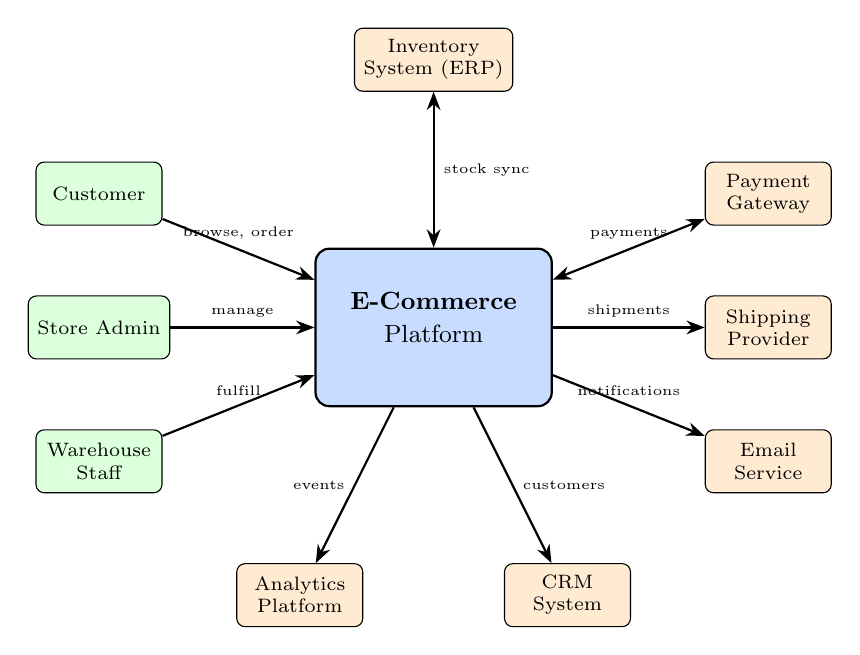
\begin{tikzpicture}[
    system/.style={draw, thick, fill=systemcolor, rounded corners=5pt, minimum width=3cm, minimum height=2cm},
    actor/.style={draw, fill=usercolor, rounded corners=3pt, minimum width=1.6cm, minimum height=0.8cm, font=\scriptsize},
    external/.style={draw, fill=externalcolor, rounded corners=3pt, minimum width=1.6cm, minimum height=0.8cm, font=\scriptsize},
    scale=0.85
]
    % System
    \node[system] (sys) at (0, 0) {};
    \node[font=\small\bfseries] at (0, 0.4) {E-Commerce};
    \node[font=\small] at (0, -0.1) {Platform};
    
    % Actors - left side
    \node[actor] (customer) at (-5, 2) {Customer};
    \node[actor] (admin) at (-5, 0) {Store Admin};
    \node[actor, align=center] (warehouse) at (-5, -2) {Warehouse\\Staff};
    
    % External systems - right side
    \node[external, align=center] (payment) at (5, 2) {Payment\\Gateway};
    \node[external, align=center] (shipping) at (5, 0) {Shipping\\Provider};
    \node[external, align=center] (email) at (5, -2) {Email\\Service};
    
    % External systems - top
    \node[external, align=center] (inventory) at (0, 4) {Inventory\\System (ERP)};
    
    % External systems - bottom
    \node[external, align=center] (analytics) at (-2, -4) {Analytics\\Platform};
    \node[external, align=center] (crm) at (2, -4) {CRM\\System};
    
    % Connections with labels
    \draw[-{Stealth}, thick] (customer) -- (sys) node[midway, above, font=\tiny] {browse, order};
    \draw[-{Stealth}, thick] (admin) -- (sys) node[midway, above, font=\tiny] {manage};
    \draw[-{Stealth}, thick] (warehouse) -- (sys) node[midway, above, font=\tiny] {fulfill};
    
    \draw[{Stealth}-{Stealth}, thick] (sys) -- (payment) node[midway, above, font=\tiny] {payments};
    \draw[-{Stealth}, thick] (sys) -- (shipping) node[midway, above, font=\tiny] {shipments};
    \draw[-{Stealth}, thick] (sys) -- (email) node[midway, above, font=\tiny] {notifications};
    
    \draw[{Stealth}-{Stealth}, thick] (sys) -- (inventory) node[midway, right, font=\tiny] {stock sync};
    
    \draw[-{Stealth}, thick] (sys) -- (analytics) node[midway, left, font=\tiny] {events};
    \draw[-{Stealth}, thick] (sys) -- (crm) node[midway, right, font=\tiny] {customers};
    
\end{tikzpicture}
\caption{E-Commerce Platform System Context Diagram}
\end{figure}

\textbf{Description:} This context diagram shows an e-commerce platform with three actor types (Customer, Store Admin, Warehouse Staff) and six external system integrations. The diagram shows data flow directions - bidirectional for payment and inventory, outbound for shipping, email, analytics, and CRM.

\subsection{Example 2: Trust Boundary Diagram}

\begin{figure}[H]
\centering
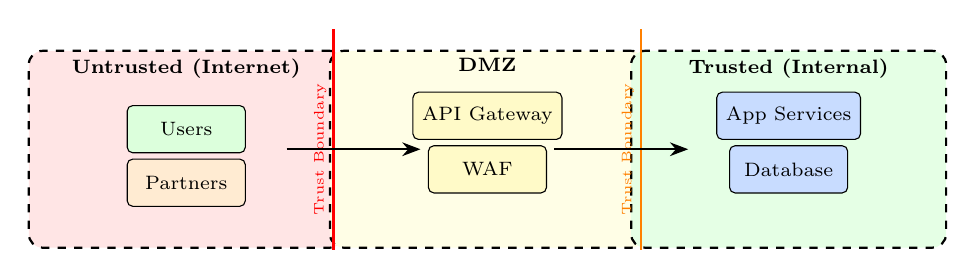
\begin{tikzpicture}[
    zone/.style={draw, thick, dashed, rounded corners=5pt, minimum width=4cm, minimum height=2.5cm},
    element/.style={draw, fill=systemcolor, rounded corners=2pt, minimum width=1.5cm, minimum height=0.6cm, font=\scriptsize},
    scale=0.85
]
    % Trust zones
    \node[zone, fill=red!10] (internet) at (-4.5, 0) {};
    \node[font=\scriptsize\bfseries, anchor=north] at (-4.5, 1.5) {Untrusted (Internet)};
    
    \node[zone, fill=yellow!10] (dmz) at (0, 0) {};
    \node[font=\scriptsize\bfseries, anchor=north] at (0, 1.5) {DMZ};
    
    \node[zone, fill=green!10] (internal) at (4.5, 0) {};
    \node[font=\scriptsize\bfseries, anchor=north] at (4.5, 1.5) {Trusted (Internal)};
    
    % Elements
    \node[element, fill=usercolor] at (-4.5, 0.3) {Users};
    \node[element, fill=externalcolor] at (-4.5, -0.5) {Partners};
    
    \node[element, fill=interfacecolor] at (0, 0.5) {API Gateway};
    \node[element, fill=interfacecolor] at (0, -0.3) {WAF};
    
    \node[element] at (4.5, 0.5) {App Services};
    \node[element] at (4.5, -0.3) {Database};
    
    % Trust boundary lines
    \draw[thick, red] (-2.3, -1.5) -- (-2.3, 1.8);
    \node[font=\tiny, red, rotate=90] at (-2.5, 0) {Trust Boundary};
    
    \draw[thick, orange] (2.3, -1.5) -- (2.3, 1.8);
    \node[font=\tiny, orange, rotate=90] at (2.1, 0) {Trust Boundary};
    
    % Flow arrows
    \draw[-{Stealth}, thick] (-3, 0) -- (-1, 0);
    \draw[-{Stealth}, thick] (1, 0) -- (3, 0);
    
\end{tikzpicture}
\caption{Trust Boundary Diagram}
\end{figure}

\textbf{Description:} This diagram shows three trust zones with different security postures. Traffic from the untrusted internet zone must pass through the DMZ (with API Gateway and WAF) before reaching internal trusted services. Each boundary crossing requires authentication and authorization.

\subsection{Example 3: Actor Catalog}

\begin{table}[H]
\centering
\caption{Actor Catalog Example}
\small
\begin{tabular}{@{}L{2cm}L{2cm}L{3.5cm}L{2.5cm}L{2.5cm}@{}}
\toprule
\textbf{Actor} & \textbf{Type} & \textbf{Primary Goals} & \textbf{Interface} & \textbf{Volume} \\
\midrule
Customer & End User & Browse products, place orders, track deliveries & Web, Mobile App & 500K MAU \\
\addlinespace
Guest & End User & Browse products, view prices & Web, Mobile App & 2M visits/mo \\
\addlinespace
Store Admin & Admin & Manage products, pricing, promotions & Admin Portal & 50 users \\
\addlinespace
Warehouse & Operator & Process orders, manage inventory & Warehouse App & 200 users \\
\addlinespace
Partner API & API Client & Sync inventory, retrieve orders & REST API & 100K req/day \\
\addlinespace
Support Agent & Operator & Handle customer issues, process refunds & Support Portal & 100 users \\
\bottomrule
\end{tabular}
\end{table}

% =============================================================================
% SECTION: NOTES
% =============================================================================
\section{Notes}

\subsection{Scope Management Best Practices}

\begin{contextbox}[Scope Definition Guidelines]
\begin{itemize}[nosep]
    \item Document scope decisions with rationale
    \item Get explicit stakeholder sign-off on boundaries
    \item Use "in/out of scope" lists for clarity
    \item Review scope at project milestones
    \item Maintain scope change control process
    \item Communicate scope to all team members
    \item Link scope to requirements traceability
\end{itemize}
\end{contextbox}

\subsection{External Dependency Management}

\begin{boundarybox}[Dependency Management Guidelines]
\begin{itemize}[nosep]
    \item Maintain an up-to-date dependency inventory
    \item Monitor external system health proactively
    \item Establish communication channels with dependency owners
    \item Plan for dependency unavailability (graceful degradation)
    \item Version external interfaces explicitly
    \item Test integration points regularly
    \item Document escalation paths for dependency issues
    \item Review dependencies for security vulnerabilities
\end{itemize}
\end{boundarybox}

\subsection{Common Pitfalls}

\begin{warningbox}[Common Mistakes to Avoid]
\begin{enumerate}[nosep]
    \item \textbf{Undefined Boundaries:} Ambiguous scope leading to feature creep
    \item \textbf{Hidden Dependencies:} Undocumented external system dependencies
    \item \textbf{Missing Actors:} Forgetting user types (auditors, support staff)
    \item \textbf{One-Way Thinking:} Not considering data flowing out of the system
    \item \textbf{Ignoring Constraints:} Not documenting regulatory or organizational limits
    \item \textbf{Optimistic SLAs:} Assuming external systems are always available
    \item \textbf{Static View:} Not planning for environment evolution
    \item \textbf{Security Afterthought:} Not identifying trust boundaries early
\end{enumerate}
\end{warningbox}

% =============================================================================
% SECTION: SOURCES
% =============================================================================
\section{Sources}

\subsection{Primary References}

\begin{enumerate}
    \item Clements, P., et al. (2010). \textit{Documenting Software Architectures: Views and Beyond} (2nd ed.). Addison-Wesley Professional.
    
    \item Brown, S. (2018). \textit{The C4 Model for Visualizing Software Architecture}. Leanpub.
    
    \item Rozanski, N., \& Woods, E. (2011). \textit{Software Systems Architecture} (2nd ed.). Addison-Wesley Professional.
    
    \item Bass, L., Clements, P., \& Kazman, R. (2021). \textit{Software Architecture in Practice} (4th ed.). Addison-Wesley Professional.
    
    \item ISO/IEC/IEEE 42010:2011. \textit{Systems and software engineering --- Architecture description}.
\end{enumerate}

\subsection{Supplementary References}

\begin{enumerate}[resume]
    \item Hohpe, G., \& Woolf, B. (2003). \textit{Enterprise Integration Patterns}. Addison-Wesley Professional.
    
    \item Vernon, V. (2013). \textit{Implementing Domain-Driven Design}. Addison-Wesley Professional.
    
    \item Newman, S. (2021). \textit{Building Microservices} (2nd ed.). O'Reilly Media.
    
    \item Richardson, C. (2018). \textit{Microservices Patterns}. Manning Publications.
    
    \item The Open Group. (2018). \textit{ArchiMate 3.1 Specification}.
\end{enumerate}

\subsection{Online Resources}

\begin{itemize}
    \item C4 Model: \url{https://c4model.com/}
    \item Arc42 Template: \url{https://arc42.org/}
    \item Structurizr: \url{https://structurizr.com/}
    \item ArchiMate: \url{https://www.opengroup.org/archimate-forum}
    \item Software Architecture Guide: \url{https://martinfowler.com/architecture/}
\end{itemize}

% =============================================================================
% APPENDIX
% =============================================================================
\appendix

\section{Context View Checklist}

\begin{table}[H]
\centering
\small
\begin{tabular}{@{}L{10cm}C{2cm}@{}}
\toprule
\textbf{Item} & \textbf{Complete?} \\
\midrule
\multicolumn{2}{l}{\textbf{Scope and Boundaries}} \\
\quad System scope clearly defined & $\square$ \\
\quad In-scope items documented & $\square$ \\
\quad Out-of-scope items documented & $\square$ \\
\quad Stakeholder agreement obtained & $\square$ \\
\midrule
\multicolumn{2}{l}{\textbf{External Actors}} \\
\quad All user types identified & $\square$ \\
\quad Actor goals documented & $\square$ \\
\quad Actor volumes estimated & $\square$ \\
\quad Interfaces for each actor defined & $\square$ \\
\midrule
\multicolumn{2}{l}{\textbf{External Systems}} \\
\quad All external systems identified & $\square$ \\
\quad System owners documented & $\square$ \\
\quad Protocols and formats specified & $\square$ \\
\quad SLAs documented & $\square$ \\
\quad Fallback strategies defined & $\square$ \\
\midrule
\multicolumn{2}{l}{\textbf{Data Flows}} \\
\quad Inbound data flows documented & $\square$ \\
\quad Outbound data flows documented & $\square$ \\
\quad Data sensitivity classified & $\square$ \\
\quad Volume estimates provided & $\square$ \\
\midrule
\multicolumn{2}{l}{\textbf{Constraints and Risks}} \\
\quad Regulatory constraints documented & $\square$ \\
\quad Technical constraints documented & $\square$ \\
\quad Dependencies assessed for risk & $\square$ \\
\quad Mitigation strategies defined & $\square$ \\
\midrule
\multicolumn{2}{l}{\textbf{Security}} \\
\quad Trust boundaries identified & $\square$ \\
\quad Authentication requirements defined & $\square$ \\
\quad Data protection requirements documented & $\square$ \\
\bottomrule
\end{tabular}
\end{table}

\section{Glossary}

\begin{description}[style=nextline, leftmargin=3cm, labelwidth=2.8cm]
    \item[Actor] A human user, role, or persona that interacts with the system.
    
    \item[API Gateway] A server that acts as a single entry point for API requests.
    
    \item[Boundary] A demarcation separating the system from its environment.
    
    \item[Constraint] A limitation imposed on the system by its environment.
    
    \item[Context] The environment in which the system operates.
    
    \item[Data Flow] Movement of data across the system boundary.
    
    \item[Dependency] A reliance on an external system or service.
    
    \item[External System] A software system outside the system boundary.
    
    \item[Interface] A point of interaction with external entities.
    
    \item[Integration] The connection between the system and external systems.
    
    \item[Scope] The extent of what is included in the system.
    
    \item[SLA] Service Level Agreement defining expected service quality.
    
    \item[Stakeholder] Anyone with an interest in the system.
    
    \item[System Under Design] The system being architected and documented.
    
    \item[Trust Boundary] A boundary separating different security trust levels.
\end{description}

% =============================================================================
% END DOCUMENT
% =============================================================================

\end{document}